\chapter{Introduction}
\label{chap:introduction}

\section{Background}
\label{sec:background}

Metabolic dysfunction-associated steatotic liver disease (MASLD), formerly
non-alcoholic fatty liver disease (NAFLD), is the most common chronic liver
disease worldwide. It affects about 30\% of the adult population, and its
prevalence has risen steadily over the past three decades
\cite{younossi2023global,riazi2022prevalence}. In 2023 a multisociety consensus
renamed the condition to reflect its metabolic origin: steatotic liver disease
accompanied by at least one cardiometabolic risk factor, such as excess
weight, raised blood glucose or dyslipidaemia \cite{rinella2023nomenclature}.
Untreated, MASLD can progress from simple fat accumulation (steatosis) to
inflammation, fibrosis and cirrhosis, and it is closely linked to type~2
diabetes and cardiovascular disease.

Diet is central to its management. No dietary pattern is a cure, but the
current European guideline recommends lifestyle change, centred on diet
quality and weight loss, as the first-line treatment for most patients
\cite{easl2024masld}. The evidence is graded by the amount of weight lost: in
a prospective study with paired liver biopsies, a loss of at least 5\% of body
weight reduced steatosis, 7--10\% improved inflammation, and 10\% or more led
to resolution of steatohepatitis in most patients and to regression of
fibrosis in many \cite{vilargomez2015weight}. Beyond weight, the guideline
advises a Mediterranean-style diet, fewer foods rich in saturated fat and
sugars, and the avoidance of sugar-sweetened beverages \cite{easl2024masld}.

Turning this guidance into daily meals is where patients struggle. Guidelines
speak in nutrients and dietary patterns (``limit saturated fat'', ``increase
fibre''), whereas people decide what to eat one recipe at a time, constrained
by the cuisine they know, the ingredients they have, the time they can spend
cooking and what they enjoy. The same advice also does not suit every
patient equally: the priority for someone whose diet is already high in fibre
but rich in saturated fat differs from that of someone with the opposite
pattern. Bridging the gap between population-level evidence and an individual
patient's plate is the problem this thesis addresses.

Liver fat itself can be measured non-invasively. Vibration-controlled
transient elastography (FibroScan) reports the controlled attenuation
parameter (CAP), which grades steatosis with established cut-offs
\cite{karlas2017cap}. The US National Health and Nutrition Examination
Survey (NHANES) performed this examination on a nationally representative
sample in its 2017--March 2020 and 2021--2023 cycles, together with blood
tests, body measurements, questionnaires and a 24-hour dietary recall
\cite{nhanes_lux}. In the 15{,}300 participants with a complete examination
used in this work, 52\% had a CAP of at least 248~dB/m, the usual threshold
for any steatosis.

\section{Digital Twins in Medicine and Nutrition}
\label{sec:digital_twins}

A digital twin is a virtual representation of a specific physical system that
is updated with data from that system, can predict how it will behave, and is
used to inform decisions about it \cite{nasem2024digitaltwins}. In medicine
the physical system is a patient, or one of their organs. Medical digital
twins are most advanced in cardiology and oncology, and their development
faces common challenges in data integration, validation and privacy
\cite{laubenbacher2024medicine,katsoulakis2024digital}. What distinguishes a
twin from a one-off prediction model is that it is specific to one patient, is
updated as new data arrive, and can simulate how that patient's state may
change under different interventions
\cite{nasem2024digitaltwins,katsoulakis2024digital}.

Nutrition is a natural application. People respond differently to the same
food \cite{zeevi2015personalized}, and the ``virtual digital twin'' concept in
precision nutrition proposes combining a person's clinical, lifestyle and
dietary data into a model that can test dietary choices before they are made
\cite{gkouskou2020virtual}. Early clinical results are encouraging: in a
one-year randomised trial in people with type~2 diabetes, nutrition guided by
a digital twin that predicted each person's post-meal glucose response
improved markers of liver fat \cite{joshi2023digitaltwin}. In MASLD
specifically, the European ARTEMIS project is building virtual twins from
retrospective data on several thousand patients \cite{artemis2024}. None of
these systems, however, evaluates complete, existing recipes against a
patient's evidence-based dietary needs.

\section{Computational Gastronomy and Recipe Data}
\label{sec:gastronomy}

Computational gastronomy treats food and cooking as data that can be analysed
and reasoned about \cite{bagler2024gastronomy}. Structured resources now make
this possible at scale. RecipeDB contains more than 118{,}000 recipes from 74
countries, each with its ingredients, cooking processes, utensils, cuisine and
nutritional profile \cite{batra2020recipedb}; FlavorDB describes the flavour
molecules found in foods \cite{garg2018flavordb}; and literature-mined
resources link culinary herbs and spices to health outcomes
\cite{rakhi2018spices}. Related work in menu planning uses multi-objective
optimisation to compose daily menus that meet nutritional targets
\cite{sahin2024menu}.

These resources are designed mainly for exploring and querying culinary data,
or for meeting generic nutrient targets. They do not, by themselves, decide
which existing recipes suit a particular patient, given that patient's
current liver state, the strength of the clinical evidence behind each dietary
change, and the practical realities of their kitchen.

\section{Problem Statement and Research Gap}
\label{sec:problem}

Three bodies of work hold complementary pieces of the problem. Clinical
evidence links dietary changes to liver outcomes; patient-specific models,
including digital twins, estimate an individual's health state; and recipe
databases describe the food people actually cook. These components are
usually studied separately. In particular, we found no framework that
evaluates and ranks existing recipes for an individual patient by combining
\begin{itemize}
    \item \textbf{health relevance}, derived from the patient's current liver
          and metabolic state and from graded intervention evidence;
    \item \textbf{cuisine compatibility}, reflecting the patient's culinary
          context; and
    \item \textbf{practical feasibility}, reflecting cooking time, number of
          ingredients and complexity,
\end{itemize}
within a transparent framework in which every recommendation can be traced
back to the evidence that supports it.

\section{Research Question and Objectives}
\label{sec:research_question}

This thesis asks:

\begin{quote}
\emph{Can a patient-specific liver digital twin, built from clinical data and
graded intervention evidence, support the evidence-grounded evaluation and
ranking of existing recipes according to their health relevance, cuisine
compatibility and cooking feasibility for an individual patient?}
\end{quote}

To answer it, the work pursues five objectives:
\begin{enumerate}
    \item Estimate each patient's current liver state, as calibrated
          probabilities of steatosis, from routinely collected clinical data.
    \item Translate that state, together with the patient's own reported
          diet, into evidence-graded nutritional priorities, without
          inventing individual numeric targets.
    \item Evaluate and rank existing recipes from RecipeDB against those
          priorities, the patient's cuisine and practical constraints.
    \item Compare recipe choices as scenarios whose projected effects are
          grounded in clinical evidence, and update the patient's state as new
          data arrive.
    \item Evaluate each component against appropriate baselines and state
          clearly what has and has not been validated.
\end{enumerate}

\section{Approach Overview}
\label{sec:approach}

The proposed system, HepatoTwin, is organised in seven layers
(Figure~\ref{fig:hepatotwin_overview}). Layer~1 holds the patient's state:
demographics, body measurements, blood tests, questionnaire answers and a
24-hour dietary recall. Layer~2, the core of the twin, estimates the current
liver state with an XGBoost model and two calibrated classifiers that give
the probability of CAP at or above 248 and 280~dB/m, explained per feature
with SHAP values. Layer~3, the evidence engine, converts this state into
nutritional priorities such as weight management or limiting saturated fat;
each priority cites rows of a curated table of 23 intervention--outcome
findings with explicit evidence-strength labels, and is adjusted by the
patient's own intake. Layer~4, the recipe evaluation and ranking engine
(NutriTwin), is the core research contribution: it scores candidate recipes
for health relevance, cuisine compatibility, practical feasibility and
acceptability, ranks first the recipes that meet every evidence-linked
reference value, and explains each recommendation. Layer~5 compares recipe
scenarios and projects their effect over time; Layers~6 and~7 present the
twin through a three-dimensional liver visualisation and an explainable
dashboard. When new measurements or food logs arrive, the twin updates its
state and its recommendations.

\begin{figure}[htbp]
    \centering
    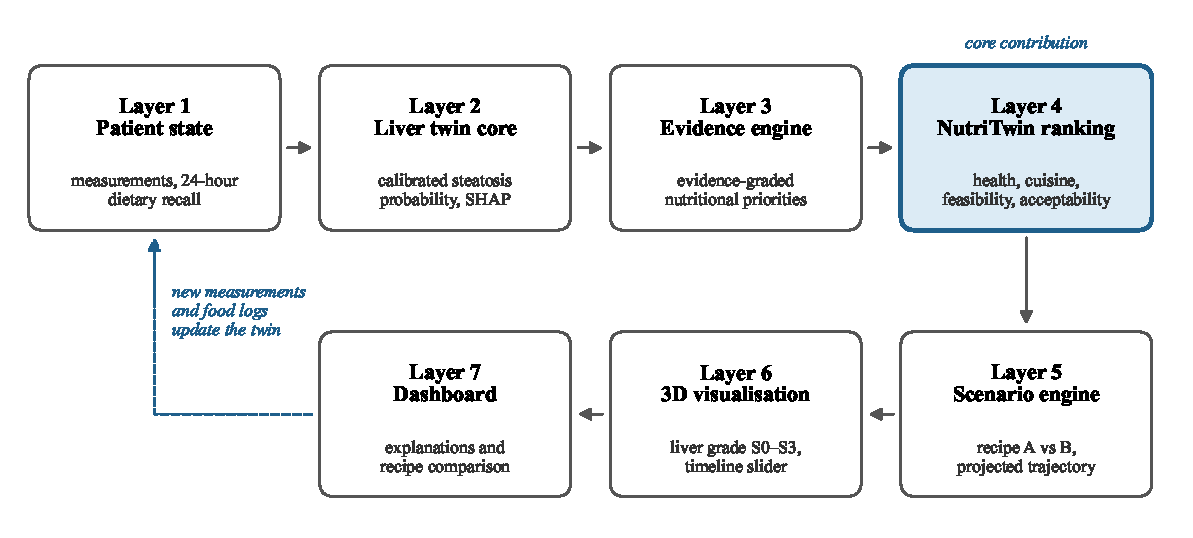
\includegraphics[width=\textwidth]{figures/hepatotwin_overview.pdf}
    \caption{Overview of HepatoTwin. The patient's data (Layer~1) feed the
             liver twin core (Layer~2), whose calibrated state drives
             evidence-graded priorities (Layer~3) and the ranking of existing
             recipes (Layer~4, the core contribution). Scenarios (Layer~5) are
             shown through a visualisation (Layer~6) and a dashboard
             (Layer~7); new measurements and food logs update the twin.}
    \label{fig:hepatotwin_overview}
\end{figure}

The twin is built and evaluated on NHANES. Its liver-state model is intended
for patients aged 12 to 59 and is evaluated against reliable FibroScan
examinations; ages 60 and over are outside its scope.

\section{Contributions}
\label{sec:contributions}

The main contributions of this thesis are:
\begin{enumerate}
    \item \textbf{A calibrated liver-state model from routine data.} Trained on
          both NHANES FibroScan cycles, the model detects steatosis with
          ROC-AUC 0.881 (CAP $\geq$ 248~dB/m) and 0.879 (CAP $\geq$ 280~dB/m)
          on held-out patients within its scope, above the Fatty Liver Index
          (0.861) and the Hepatic Steatosis Index (0.836) on the same patients
          \cite{bedogni2006fli,lee2010hsi}, and holds its performance on a
          later survey cycle. It also predicts CAP with a held-out R$^2$ of
          0.56, comparable to or above published models built on routine data.
    \item \textbf{An evidence engine linking patient state to graded dietary
          priorities.} Every priority cites named trials, meta-analyses or
          guidelines with an explicit strength label, observational findings
          are recorded but never used as effects, and the patient's own
          24-hour recall personalises the priorities.
    \item \textbf{NutriTwin, an evidence-gated multi-criteria recipe ranking
          engine.} On 300 held-out patients, 83\% of its top-ten recipes met
          every evidence-linked reference value, the patient's cuisine and the
          practical limits at once, against 73\% for weighted scoring without
          the health gate and under 2\% for health-only ranking; it was the
          only method whose recommendations always met the nutritional
          references.
    \item \textbf{Scenario comparison and weekly meal plans} that respect the
          patient's cuisine and nutritional references, with projected effects
          labelled by the strength of their evidence.
    \item \textbf{An open, modular digital-twin framework}, demonstrated for
          MASLD, together with an in-silico evaluation design that tests how
          the twin updates on virtual patients before real follow-up data
          exist.
\end{enumerate}

\section{Scope and Limitations}
\label{sec:scope}

NHANES is cross-sectional: each participant was examined once. The twin's
estimate of the current state is therefore validated on held-out patients,
but its projections of future states cannot be compared with real repeat
measurements. They are presented as simulated projections grounded in
clinical evidence, never as clinical forecasts, and the twin's updating is
evaluated on virtual patients. Validation with real longitudinal data
requires deployment with patients who enter their own measurements over
time. The recommendations are research outputs: they support, and do not
replace, clinical care.

\section{Thesis Outline}
\label{sec:outline}

Chapter~2 reviews related work on MASLD and its dietary treatment,
non-invasive liver fat assessment, machine-learning prediction of steatosis,
dietary assessment, digital twins, computational gastronomy and the
evaluation of twins without longitudinal data. Chapter~3 describes the
methodology: the NHANES cohort and the recipe corpus, the liver-state model,
the evidence engine, the recipe evaluation and ranking engine, and the
scenario and updating components of the twin. Chapter~4 reports the
experiments carried out to improve the prediction of CAP, and explains why
its performance reaches a plateau. Chapter~5 presents the results of each
component against its baselines.
